\section{Results and Analysis}
\subsection{Evaluation measures}
We evaluated image recognition, task execution and final placement separately. The detection metrics below describe model predictions; physical sorting results come from the videos and task records.

For detection, precision and recall can be written as
\begin{equation}
P=\frac{TP}{TP+FP},\qquad R=\frac{TP}{TP+FN},
\end{equation}
where $TP$ is a correct detection, $FP$ is a false detection, and $FN$ is a missed target under the evaluation matching rule. Precision helps describe false-target pressure; recall helps describe how many targets are found. Both are relevant to sorting. A false target may cause an unnecessary pick, while a missed object may remain on the table.

The overlap between a predicted box $B$ and a reference box $G$ is
\begin{equation}
\operatorname{IoU}(B,G)=\frac{|B\cap G|}{|B\cup G|}.
\end{equation}
mAP50 summarizes average precision with an IoU matching threshold of 0.50. mAP50--95 averages results over thresholds from 0.50 to 0.95 in steps of 0.05. The detector's mAP and the robot's transfer success rate measure different stages of the system.

\subsection{Simulation workflow results}
The final HSV simulation sorted four cubes and two bridges correctly: 6/6 total and 2/2 bridges. Independent acceptance recorded 37,831 joint samples, no joint-limit violations, no monitored unsafe contact pairs, and 391.53 s. Section~\ref{sec:simulation} provides all six object-level results and saved evidence.\src{simbridgerun}

The two geometries completed the same pickup and placement sequence. The HSV detector and fixed-constraint grasp model are described in the simulation chapter.

\subsection{Offline model results}
The model results available from training and the defense presentation are listed below. The v3 baseline includes four metrics; the v4 result gives mAP50--95.\src{defense}

\begin{table}[H]\tabstart
\caption{Detector results reported in the defense presentation}
\begin{tabularx}{\textwidth}{@{}L{3.8cm}*{4}{>{\centering\arraybackslash}X}@{}}
\toprule Model and source & Precision & Recall & mAP50 & mAP50--95\\\midrule
v3 baseline, slide 9 & 0.9505 & 0.9342 & 0.9360 & 0.8699\\
Final v4, slide 4 & Not stated & Not stated & Not stated & 0.8755\\
\bottomrule
\end{tabularx}
\end{table}

The recorded mAP50--95 increased from 0.8699 to 0.8755, a difference of 0.56 percentage points. The v4 training added field images and difficult backgrounds. The available summary results do not isolate the contribution of individual training changes.

The red/pink classifier achieved 94.12\% Top-1 accuracy on 68 test crops: 26 pink and 42 red. In the running pipeline, it changes a pink prediction to red only when its score reaches the configured threshold. The crop test does not include missed detections or grid-assignment errors.\src{classifiermetrics}

\subsection{Physical sorting demonstration}
With the instructor's approval, we started the physical test with five objects and re-fed the yellow cube once, producing six transfers. The acceptance video shows the red cuboid, yellow cube, re-fed yellow cube, blue cube, orange bridge, and green cube delivered to their corresponding sorting areas. Four cube transfers go right and two non-cube transfers go left. All six transfers went to the intended sorting area; the group recorded no failed transfer.\src{physicalvideo}
\begin{equation}
S_{\mathrm{cycles}}=\frac{6\text{ matching destination choices}}{6\text{ transfer cycles}}=100\%.
\end{equation}

\begin{table}[H]\tabstart
\caption{Observed acceptance-video cycles}\label{tab:physicalobjects}
\begin{tabularx}{\textwidth}{@{}L{1.2cm}Y L{1.5cm}L{2.9cm}L{3cm}@{}}
\toprule Cycle & Visible object & Area & Grasp/transport & Delivery interval\\\midrule
P01 & Red cuboid & Left & Observed & 00:22--00:25\\
P02 & Yellow cube & Right & Observed & 01:16--01:19\\
P03 & Re-fed yellow cube & Right & Observed & 02:04--02:06\\
P04 & Blue cube & Right & Observed & 02:48--02:49\\
P05 & Orange bridge & Left & Observed & 03:22--03:24\\
P06 & Green cube & Right & Observed & 03:59--04:01\\
\bottomrule
\end{tabularx}
\end{table}
The intervals refer to \file{2eb7001d38fd861630d52918161ba8cf.mp4} and use approximate playback timestamps. The operator re-feeds the yellow cube and clears delivered objects. Cycle IDs describe transfer order rather than six distinct physical objects.

\begin{figure}[H]
\centering
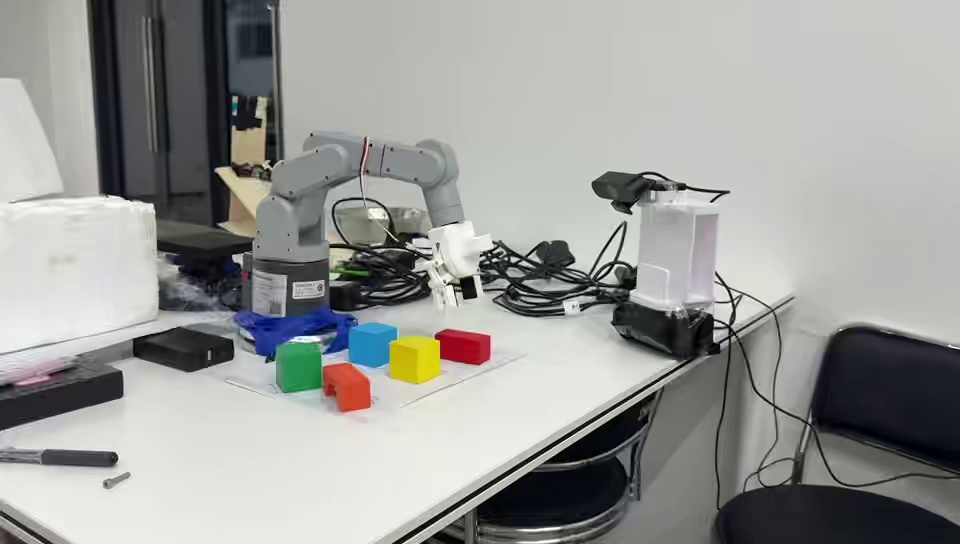
\includegraphics[width=0.47\textwidth]{figures/physical_acceptance_initial.jpg}\hfill
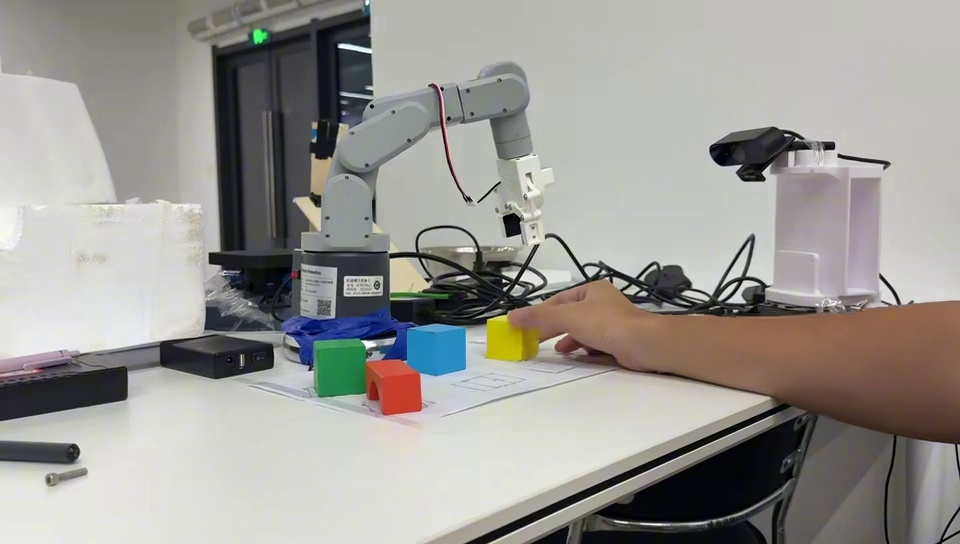
\includegraphics[width=0.47\textwidth]{figures/physical_acceptance_refeed.jpg}
\caption{Physical acceptance: initial scene and yellow-cube re-feed at approximately 01:24.}
\end{figure}

\subsection{Original task records}
The task JSONL for 2026-09-08 03:25:15 records an armed controller, six transfer requests, six completed worker results, six accepted transfers, and final \file{completed_count=6}. Its chronological source grids are G1, G3, G2, G4, G5, and G6. Request IDs connect source selection, destination, worker feedback, and source-clear verification.\src{physicalrecords}

\begin{table}[H]\tabstart
\caption{Six-cycle task log}
\begin{tabularx}{\textwidth}{@{}L{1.4cm}L{1.4cm}Y L{2cm}L{2.6cm}@{}}
\toprule Request & Grid & Recorded detector label & Area & Worker result\\\midrule
1 & G1 & \file{orange_bridge} & Left & COMPLETED\\
2 & G3 & \file{yellow_cube} & Right & COMPLETED\\
3 & G2 & \file{yellow_cube} & Right & COMPLETED\\
4 & G4 & \file{blue_cube} & Right & COMPLETED\\
5 & G5 & \file{orange_bridge} & Left & COMPLETED\\
6 & G6 & \file{green_cube} & Right & COMPLETED\\
\bottomrule
\end{tabularx}
\end{table}
The table lists detector outputs. The video table above instead describes visible object shapes and playback times; the source files are identified with each record.

The v4 task of 2026-09-07 19:26:01 is a separate five-transfer run, covering G1, G2, G3, G5, and G6. G4 remained without a stable target. Its final count is five. The matching visual-recognition AVI shows the detector overlays and five-object scene; these records are not added to the six-cycle total.

\subsection{Empty and unknown targets}
Recovered physical-unknown tests at 15:38:52 and 19:50:38 on September 7 record G1 as \file{UNKNOWN} and then \file{SKIP_NO_MOTION}, with no transfer request. Empty cells are also skipped. Both tests use a disarmed controller to inspect the visual and task-decision branches. An additional interface-injection test records the unsupported-class path. Original JSONL, console outputs, and evidence images are included.\src{physicalrecords}

\subsection{Red-cuboid and orange-bridge refinement}
The detector includes a \file{red_orange_pair_classifier_v2.pt} stage for candidates labelled \file{red_cuboid} or \file{orange_bridge}. A result is accepted when its confidence is at least 0.80 and its lead over the second class is at least 0.30. Otherwise, the main detector label is retained. This refinement changes the fine class while preserving the shared left-side sorting group.\src{pairrefinement}

The classifier test produced 84/84 correct crops. In a video regression of 36 detections, 20 red-cuboid cases change from bridge labels to red-cuboid labels, and 16 bridge cases remain correct. Both evaluations used saved image data; the updated classifier has not been evaluated in a new physical acceptance run.

\subsection{Operating settings}
The main detector confidence is 0.25; NMS IoU is 0.45. Detection-box centers determine unique polygon ownership. A seven-observation history requires at least five matching sorting-group votes, with the current group also matching before a target is ready. The controller routes \file{cube} right and \file{other} left.\src{controller,integration}

The classification gripper profile is \file{OPEN=100}, \file{cube CLOSE=69}, \file{other CLOSE=40}, and speed 20. The calibration files provide 17 measured reference poses and directional correction data. Before operation, the region layout and poses are checked against the current setup.\src{motion,gripper}

